%!TEX root = forallx-adl.tex
\part{The Language of Sentential Logic}
\label{ch.TFL}
\addtocontents{toc}{\protect\mbox{}\protect\hrulefill\par}

\chapter{First Steps to Symbolisation}\label{s:firststeps}

\section{Argument Structure}\label{s:ValidityInVirtueOfForm}
Consider this argument:
	\begin{earg}
		\item[] It is raining outside.
		\item[] \textsf{If} it is raining outside, \textsf{then} Jenny is miserable.
		\item[So:] Jenny is miserable.
	\end{earg}
and another argument:
	\begin{earg}
		\item[] Jenny is an anarcho-syndicalist.
		\item[] \textsf{If} Jenny is an anarcho-syndicalist, \textsf{then} Dipan is an avid reader of Tolstoy.
		\item[So:] Dipan is an avid reader of Tolstoy.
	\end{earg}
Both arguments are valid, and there is a straightforward sense in which we can say that they share a common structure. We might express the structure thus, when we let letters stand for phrases in the original argument:
	\begin{earg}
		\item[] A
		\item[] \textsf{If} A, \textsf{then} C
		\item[So:] C
	\end{earg}
This is an excellent argument \define{structure}. Surely any argument with \emph{this} structure will be valid. And this is not the only good argument structure. Consider an argument like:
	\begin{earg}
		\item[] Jenny is \textsf{either} happy \textsf{or} sad.
		\item[] Jenny is \textsf{not} happy.
		\item[So:] Jenny is sad.
	\end{earg}
Again, this is a valid argument. The structure here is something like:
	\begin{earg}
		\item[] A \textsf{or} B
		\item[] \textsf{not}: A
		\item[So:] B
	\end{earg}
A superb structure! You will recall that this was the structure we saw in the original arguments which introduced the idea of validity in §\ref{s:validityintro}. And here is a final example:
	\begin{earg}
		\item[] \textsf{It's not the case that} Jim \textsf{both} studied hard \textsf{and} acted in lots of plays.
		\item[] Jim studied hard
		\item[So:] Jim did \textsf{not} act in lots of plays.
	\end{earg}
This valid argument has a structure which we might represent thus:
	\begin{earg}
		\item[] \textsf{not both}: A \textsf{and} B
		\item[] A
		\item[So:] \textsf{not}: B
	\end{earg}
The examples illustrate the idea of validity – conclusiveness in virtue of structure. The validity of the arguments just considered has nothing very much to do with the meanings of English expressions like `Jenny is miserable', `Dipan is an avid reader of Tolstoy', or `Jim acted in lots of plays'. If it has to do with meanings at all, it is with the meanings of phrases like `and', `or', `not,' and `if …, then …'.

\section{Sentence Trees and Canonical Clauses}\label{ss.canonical}

Since arguments are made of sentences, the logical structure of an argument will be related to the grammatical structure of the sentences within it. We've already seen in §\ref{s:truthvalues} that arguments are made up of declarative sentences. One standard way of analysing the grammatical structure of a declarative sentence is to break it into constituent phrases. Such approaches are known as  \define{phrase structure grammars}. These structures are usefully depicted in a hierarchical \define{syntactic tree}. Consider the example: \begin{earg}
	\item[\ex{tariq}] Tariq is a man.
\end{earg} This sentence (phrase of type S) can be divided into two main parts: the \define{noun phrase} `Tariq' (type NP), and the \define{verb phrase} `is a man' (type VP). In this example, the verb phrase itself divides into the verb `is' and the \define{determiner phrase} `a man' (type DP). We will return to the internal structure of sentences in §\ref{s:FOLBuildingBlocks}. This phrase structure is depicted in the tree in Figure \ref{fig:tariq}.
\begin{figure}
\begin{tikzpicture}[sibling distance=16pt]
	\Tree [.S [.NP Tariq ] [.VP is [.DP a man ] ] ]
\end{tikzpicture}
\caption{A phrase structure tree for Example \ref{tariq}. \label{fig:tariq}}
\end{figure}

Let's look at a more complicated example. Consider \begin{earg}
	\item[\ex{alice}] Alice will ace the test, or Bob will.
\end{earg} First we note that this sentence is elliptical, the verb phrase `ace the test' being omitted after `Bob will' as it is understood to be supplied by the first clause of the sentence.\footnote{A closely related example is discussed by Paul Elbourne (2011) \emph{Meaning}, Oxford University Press, pp.\ 74–6. He argues that this kind of elision is crucial evidence for phrase structure grammars, for only phrases can be omitted in this way: witness the ungrammatical `Alice will ace the test and Bob will the', where arbitrary words are omitted that do not form a grammatical phrase. This is evidence that English syntax is sensitive to the phrasal structure of sentences, and does not treat them as merely a string of words.} The full tree, with the elided phrase supplied (marked by having the VP label in a box at the lower right), is depicted in Figure \ref{fig:alice}. In this example, the whole sentence is a compound of two clauses which are sentences in their own right, or \define{subsentences}, connected by `or'.
\begin{figure}
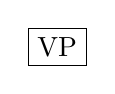
\begin{tikzpicture}[sibling distance=13pt]
 	\Tree [.S [.S [.NP Alice ] [.VP will [.VP ace [.DP the test ] ] ] ] [ [.Coord or ] [.S [.NP Bob ] [.VP will [.\node[draw]{VP}; \edge[roof]; {ace the test}  ] ] ] ] ]
 \end{tikzpicture} 	\caption{A phrase structure tree for Example \ref{alice}. \label{fig:alice}}
\end{figure} 

When analysing the structure of compound sentences, a useful notion is that of a \define{canonical clause}.\footnote{A fuller treatment of canonical clauses can be found in Rodney Huddleston and Geoffrey Pullum (2005) \emph{A Student's Introduction to English Grammar}, Cambridge University Press, pp.\ 24–5.} These are the simplest units of English sentences that can constitute a sentence by themselves. Here are some examples: 
\begin{earg}
	\item[\ex{cc1}] They knew the victim.
	\item[\ex{cc3}] She has read your article.
	\item[\ex{cc2}] Jenny is happy.
\end{earg}
A canonical clause has internal structure too, but its parts are not themselves sentences. It is composed of a \define{grammatical subject}, typically but not always a noun phrase (`Jenny', `She'), and a \define{predicate}, always a verb phrase (`knew the victim', `is happy'). 

The following, in contrast with the previous examples, are noncanonical clauses: 
\begin{earg}
	\item[\ex{nc1}] They \underline{did not} know the victim.
	\item[\ex{nc3}] She has read your article \underline{and} she vehemently disagrees with it.
	\item[\ex{nc2}] She says that \underline{Jenny is happy}.
\end{earg} These give us some characteristics of canonical clauses:
\begin{itemize}
	\item They are \emph{positive}, as in \ref{cc1}, rather than negative, as indicated by the underlined `not' in \ref{nc1}.
	\item Canonical clauses are simple, and not coordinated with any other clause, as in \ref{cc3}. In \ref{nc3}, the \define{coordinator} `and' links two clauses that would be canonical on their own into a longer \define{compound} sentence.
	\item The underlined clause in \ref{nc2} is a \emph{subordinate} clause, part of a more complex clause. Canonical clauses are main clauses, as in \ref{cc2}.
\end{itemize}

\section{Identifying Argument Structure}\label{ss.idargstr}

Our topic is not English grammar. But the idea of a canonical clause is illuminating for the logic we are examining in this part of the course. Sentential logic is, more or less, the logic that helps us understand and analyse arguments whose conclusiveness depends on their constituent canonical clauses and how they are joined together by \define{sentence connectives}. The sentence connectives we focus on are a grammatically diverse group, including \begin{description}
	\item[Coordinators] including ‘and’, ‘or’, ‘if and only if ’ (also ‘but’)\item[Adjunct heads] including ‘if … then …’, ‘only if’ (also ‘unless’, ‘because’, ‘since’, ‘hence’ – though we treat these last as signalling premises and conclusions of arguments)
	\item[Negatives] including ‘not’, ‘‐n’t’, ‘it is not the case that’ (‘never’).
	\item And there are others that we won’t deal with (‘always’, ‘might’).
\end{description}


How can we identify the logical structure of an argument? The logical structure of an argument is the form one arrives at by `abstracting away' the details of the words in an argument, \emph{except for a special set of words}, the \define{structural words}. This connects with what we have just been saying, because in many of the examples from §\ref{s:ValidityInVirtueOfForm}, the arguments can be analysed as involving canonical clauses which are linked by the structural words `and', `or', `not', `if … then …' and `… if and only if …'. So our efforts to identify the logical structure of arguments often coincide with linguist's efforts to identify the canonical clauses that constitute the sentences in those arguments – or, at least, constitute some plausible paraphrase or reformulation of those sentences.

We can see this if we return to this earlier argument: \begin{earg}
	\item[] Jenny is either happy or sad.
	\item[] Jenny is not happy.
	\item[So:] Jenny is sad.
\end{earg}
We paraphrase the compound sentence `Jenny is either happy or sad' into a compound of two canonical clauses, joined by the coordinator `or':
\begin{itemize}
\item Jenny is happy or Jenny is sad.
\end{itemize} 
And we paraphrase the noncanonical clause `Jenny is not happy' as the negative clause 
\begin{itemize}
	\item It is not the case that: Jenny is happy.

	\end{itemize} Identifying the coordinator `or' and the negative clause `it is not the case that' as structural words, and replacing the canonical clause `Jenny is happy' with the placeholder letter `A', and the canonical clause `Jenny is sad' with the placeholder letter `B', we arrive again at the argument structure we previously identified:
	\begin{earg}
		\item[] A \textsf{or} B
		\item[] \textsf{not}: A
		\item[So:] B
	\end{earg}

In this and the other examples above, we removed all details of the arguments except for the special words `and', `or', `not' and `if …, then …', and replaced the other clauses in the argument (or its near paraphrase) by placeholder letters `A', `B', etc. (We were careful to replace the same clause by the same placeholder every time it appeared.)

Another example: \begin{earg}
	\item[\ex{pst1}] Butter isn't healthy, but it is delicious.
\end{earg} We begin by paraphrasing. We note that the pronoun `it' is actually referring to the previously mentioned subject `butter', and we move the negative `isn't' into a position that reveals the canonical clause `butter is healthy'. We also note that the effect of `but' is roughly the same as our structural word `and' (though it suggests a contrast that `and' does not, `but' expresses the roughly equivalent idea that each of the claims it connects are true) we obtain this more stilted paraphrase: \begin{earg}
	\item[\ex{pst2}] It is not the case that butter is healthy and butter is delicious.
\end{earg} This paraphrase has the syntactic tree in Figure \ref{fig:butter}. \begin{figure}
	\begin{tikzpicture}
		\Tree [.S [.S Not  [.S \edge[roof]; {butter is healthy} ] ] [  and  [.S \edge[roof]; {butter is delicious} ] ] ]
	\end{tikzpicture}
	\caption{Paraphrase of Example \ref{pst1} showing its subsentential structure, as in Example \ref{pst2}.\label{fig:butter}}
\end{figure} Note that we have not further broken down the canonical clauses into subject-predicate form, because our structural words, the sentence connectives, do not occur within any canonical clause and hence are not `visible' to our analysis at the level of sentences. Finally, we replace the canonical clauses with placeholder sentences, and we reach the structure `Not A and B'.

The schematic paraphrase `Not A and B' is potentially ambiguous, because it is not obvious whether the `not' applies just to the A-clause, or to the whole `A and B' clause. We could introduce parentheses to eliminate this ambiguity, distinguishing `Not (A and B)' from `Not A and B'. This is the approach we will take in our formal language \TFL (see page \pageref{p.con.ambig}). Alternatively, we can use the hierarchical nature of syntactic trees to see see that there are two different structures possible for `Not A and B', as depicted in the schematic syntactic trees in Figure \ref{fig:butter2}. \begin{figure}
	\begin{tikzpicture}[sibling distance=16pt]
		\Tree [.S [.S Not  [.S A ] ] [  and  [.S B ] ] ]
	\end{tikzpicture}
		\begin{tikzpicture}[sibling distance=16pt]
		\Tree [.S Not [.S [.S A ]  [ and  [.S B ] ] ] ]
	\end{tikzpicture}
	\caption{Different sentential structures for `Not A and B' shown in schematic syntactic trees.\label{fig:butter2}}
\end{figure}


Sharp-eyed readers will have noticed that our list of special words doesn't precisely line up with the canonical clauses we introduced in §\ref{ss.canonical}. Consider the noncanonical clause `She said that Jenny is sad', in which the canonical clause `Jenny is sad' is subordinate within an indirect speech report. Because `She said that' is not on our special list of words, we cannot analyse this sentence as composed from a canonical clause and some structural expression. So for the purposes of sentential logic, we will treat `She said that Jenny is sad' \emph{as if} it were canonical, even though it is not from the point of view of English grammar. From the point of view of our structural words, this sentence doesn't have any further structure that we can identify. Such \define{quasi-canonical clauses} – clauses that do not feature any of our list of structural words – will also be replaced by placeholder letters in our analysis. 


This raises another question. What makes the words on our list special? Logicians tend to take a pragmatic attitude to this question. They say: \emph{nothing}! If you had chosen different words, you would have come up with a different structure. In terms of the syntactic trees we drew above, there is a hierarchy of levels when breaking down the top-level sentence into constituent phrases, and different choices of structural words correspond to different choices concerning the level at which to stop our analysis.

Linguists take a very expansive view of structural words, so that the class of canonical clauses is rather small, and there is a lot of structure to be identified in natural language. For example, the presence of modal auxiliaries (like `will' or `must', as in `James \underline{must} eat'), verb inflections other than the present tense (e.g., `they \underline{took} snuff'), and subordination (as in `\underline{Etta knew that} peaches were abundant'), in addition to items on our list of structural words, suffices to make a clause noncanonical. And there are logics which do take these to be structural words: modal logics, tense logics, and epistemic logics treat these as structural words and provide recipes for the structural analysis of arguments that abstract away features other than these words. But there is no fundamental principle that divides words once and for all into structural words and other words. So logicians are more interested in quasi-canonical clauses, given some fixed list of structural words, when using logic to model or represent natural languages. 

We will start simply, and focus on the list of truth-functional sentence connectives, principally `and', `or', `not', `if … then …' and `… if and only if …'. There are practical reasons why these words are useful ones to focus on initially, which I will now discuss.

\section{Formal Languages}

In logic, a \define{formal language} is a language which is particularly suited to representing the structure or form of its sentences. Such languages have a precisely defined \define{syntax}, that allows us to specify without difficulty the grammatical sentences of the language, and they also have a precise \define{semantics} which both tells us what meanings \emph{are} in those languages, and assigns meanings to the sentences and their constituents. 

Formal languages are not the same as natural languages, like English. The languages we will be looking at are much more limited in their expressive power than English, and not subject to ambiguity or imprecision in the way that English is. But a formal language can be very useful in \emph{representing} or modelling features of natural language. In particular, they are very good at capturing the \emph{structure} of natural language sentences and arguments, because we can design them specifically to represent a particular level of structural analysis. The semantics we give for such languages reflects that this is their primary use, as you will see. The languages assign fixed meanings only to those expressions which can be used to represent structure, but (unlike English) not every expression is treated as structural.

In this chapter we will begin developing a formal language which will allow us to represent many sentences of English, and arguments involving those sentences. The language will have a very small basic vocabulary, since we are designing it to represent the sentential structure of the examples with which we began. So it will have expressions corresponding to the English sentence  connectives `and', `or', `not' and `if …, then …' and `if and only if'. The language represents these English connectives by its own class of dedicated sentence connectives which allow simple sentences of the language to be combined into more complex sentences. These words are a good class to focus on in developing a formal language, because languages with expressions analogous to these feature a good balance between being useful and being well behaved and easy to study. The language we will develop is called \TFL, and the study of that language and its features is called \emph{sentential logic}. (It also has other names: see Appendix~\ref{app.notation}.) 

Once we have our formal language \TFL, we will be able to go on (in chapter \ref{ch.TruthTables}) to show that it has a very nice feature: it is able to represent the structure of a large class of valid natural language arguments. So while logic can't help us with every good argument, and it can't even help us with every conclusive argument, it can help us to understand arguments that are valid, or conclusive due to their structure, when that structure involves  `and', `or', `not', `if' and various other expressions. 

We will see later in this book that one could take additional  expressions in natural language to be involved is determining the structure of a sentence or argument. The language we develop in chapter~\ref{ch.FOL} is one that is suited to represent what we get when we take names like `Juanita', predicates like `is a vixen' or `is a fox', and quantifier expressions like `every' and `some' to be structural – see also §\ref{s:MoreMonadic}. And as we have mentioned, there are still other formal logical languages, unfortunately beyond the scope of this book, which take still other words or grammatical categories as structural: logics which take modal words like `necessarily' or `possibly' as structural, and logics which take temporal adverbs like `always' and `now' as structural.\footnote{Some arguments will be valid in richer logical frameworks, but not according to the more austere framework for logical structure provided by \TFL. For example `Sylvester is always active; so Sylvester is active now' is conclusive. From the point of view of temporal logic, the argument has this form `Always A; so now A', which is valid in normal temporal logics. But it is not valid according to \TFL, because the premise `Sylvester is always active' has no internal structural words that occur on the list of sentence connectives that \TFL\ represents.} What we notice here is that using logic to model natural language arguments inevitably involves a compromise. If we have lots of structural words, we can show many conclusive arguments to be valid, but our logic is complex and involves many different sentence connectives. If we take relatively few words as structural, we can represent fewer conclusive arguments as valid, but our formal language is a lot easier to work with. 

We will start now by putting those tantalising observations about richer logics out of your mind! We'll focus to begin with on the language \TFL, and on how we can use it to model arguments in English featuring some particular sentence connectives as structural words, including those we've just highlighted above. This collection of structural words has struck many logicians over the years as providing a good balance between simplicity and strength, ideal for an introduction to logic.


\section{Atomic Sentences}
In §\ref{s:ValidityInVirtueOfForm}, we started isolating the form of an argument by replacing quasi-canonical clauses (those including none of our list of structural words) within the argument with individual placeholder letters. Thus in the first example of this section, `it is raining outside' is a quasi-canonical clause of `If it is raining outside, then Jenny is miserable', and we replaced this clause with `A'. 

Our artificial language, \TFL, pursues this idea absolutely ruthlessly. We start with some \define{atomic sentences}, which are analogues of the canonical clauses of natural languages.  These will be the basic building blocks out of which more complex sentences are built. Unlike natural languages, these simplest sentences of \TFL\ have no interesting internal structure at all. The atomic sentences of \TFL\ will consist of upper case italic letters, with or without numerical subscripts. There are only twenty-six letters of the alphabet, but there is no limit to the number of atomic sentences that we might want to consider, so we add numerical subscripts to each letter to extend our library of atomic sentences indefinitely. This procedure does give us atomic sentences with some syntax, but it is irrelevant to meaning: there is no connection between `$A_{8}$' and `$A_{67}$' just because they both involve `$A$'. Likewise, there is no connection between `$D_{17}$' and `$G_{17}$' even though they share the same numerical subscript. Upper case italic letters, with or without subscripts, are all the atomic sentences there are. So, here are five different atomic sentences of \TFL:
	$$A, P, P_{1}, P_{2}, A_{234}.$$ 

Atomic sentences are the basic building blocks of \TFL. But what motivates their introduction is the fact that they can be used to represent, or \emph{symbolise}, certain English sentences. To do this, we provide a \define{symbolisation key}, such as the following, which assigns a temporary linkage between some atomic sentences of \TFL, and some quasi-canonical sentences of the natural language we are representing using \TFL, in this case, English:
	\begin{ekey}
		\item[A] It is raining outside.
		\item[C] Jenny is miserable.
	\end{ekey}
In doing this, we are not fixing this symbolisation \emph{once and for all}. We are just saying that, for the time being, we shall use the atomic sentence of \TFL, `$A$', to symbolise the English sentence `It is raining outside', and the atomic sentence of \TFL, `$C$', to symbolise the English sentence `Jenny is miserable'. Later, when we are dealing with different sentences or different arguments, we can provide a new symbolisation key; as it might be:
	\begin{ekey}
		\item[A] Jenny is an anarcho-syndicalist.
		\item[C] Dipan is an avid reader of Tolstoy.
	\end{ekey}
Given this flexibility, it isn't true that a sentence of \TFL\ \textbf{means the same thing} as any particular natural language sentence – see also §\ref{sec:symvstrans}. The question of what any given atomic sentence of \TFL\ means is actually a bit hard to make sense of; we will return to it in §\ref{s:CompleteTruthTables}.


But it is important to understand that whatever internal structure an English sentence might have is lost when it is symbolised by an atomic sentence of \TFL. From the point of view of \TFL, an atomic sentence is just a letter. It can be used to build more complex sentences, but it cannot be taken apart. So we cannot use \TFL\ to symbolise arguments whose validity depends on structure within sentences that are symbolised as atomic sentences of \TFL, such as arguments whose conclusiveness turns on different structural words than those \TFL\ seeks to capture, or arguments which depend on the internal subject-predicate structure of canonical clauses.





\keyideas{
	\item Arguments are made of sentences, and to understand the structure of an argument we must understand the syntactic structure of those sentences, including analysing those sentences into their simplest constituents, roughly, how a compound sentence can be constructed by combining canonical clauses. 
	\item The formal language \TFL\ is designed to model English arguments involving compound sentences structured by the sentence connectives `and', `or', `not', and `if', and related expressions.
	\item We symbolise these arguments this by abstracting away any other aspects of English sentences, using structureless atomic sentences to represent clauses that do not include these special expressions.
	\item Many English words and phrases could be treated as structural, and different formal languages can be motivated by other views about the structure of natural language sentences. But \TFL\ represents a particularly well behaved aspect of English sentence structure.
}

\practiceproblems

\problempart True or false: if you are going to represent an English sentence by an atomic sentence in Sentential, the English sentence cannot have a sentence connective (like ‘and’) occurring within it.

\problempart Which one or more of the following are \textbf{not} atomic sentences of \TFL? \begin{earg}
	\item $A'$;
	\item $W_{0}$;
	\item $Q_{5902222}$;
	\item $77_{P}$;
	\item $V^{9}$.
\end{earg}

\problempart This argument is invalid in English: `There is water in the glass and it is cold; therefore it is cold'. Comment on why it is invalid, and what potential pitfalls arise when considering how to symbolise this argument into \TFL. 


\chapter{Connectives}\label{s:TFLConnectives}
In the previous section, we considered symbolising relatively simple English sentences with atomic sentences of \TFL, when they did not include any of our list of structural words, the English sentence connectives `and', `or', `not', and so forth. This leaves us wanting to deal with sentences including these structural words. In \TFL, we shall make use of logical connectives to build complex sentences from atomic components. There are five logical connectives in \TFL, inspired by the English structural words we have encountered so far. This table summarises them, and they are explained throughout this section. 

	\begin{table}[h]
	\center
	\begin{tabular}{l l l} \toprule 
	
	\textbf{Symbol}&\textbf{What it is called}&\textbf{Rough English analogue}\\
	\midrule
	\enot&negation&`It is not the case that $…$'\\
	\eand&conjunction&`Both $…$\ and $…$'\\
	\eor&disjunction&`Either $…$\ or $…$'\\
	\eif&conditional&`If $…$\ then $…$'\\
	\eiff&biconditional&`$…$ if and only if $…$'\\
	
	\bottomrule \end{tabular}
	\end{table}

As the table suggests, we will introduce these connectives by the English connectives they parallel. It is important to bear in mind that they are perfectly legitimate standalone expressions of \TFL, with a meaning independent of the meaning of their English analogues. The nature of that meaning we will see in §\ref{s:CompleteTruthTables}. \TFL\ is not a strange way of writing English, but a free-standing formal language, albeit one designed to represent some aspects of natural language.

\section{Modelling and Paraphrase} % (fold)
\label{sec:modelling_and_paraphrase}

We saw in §\ref{ss.idargstr} the grammatical heterogeneity of the sentence connectives. Even within the same class of connective we don't have grammatical uniformity. The different sentence connectives that express negation – e.g., `not', `-n't', and `it is not the case that' – can occur in quite different places in a grammatical sentence. Consider these examples:
 \begin{earg}
	\item Vassiliki doesn’t like ballet;
	\item Vassiliki dislikes ballet;
	\item It is not the case that Vassiliki likes ballet.
\end{earg} To the grammarian, these differences are of great significance. To the logician, they are not. When the logician considers these examples, what matters is that these are all negated sentences, not the particular way that the idea of negation happens to be implemented syntactically in English. All these sentences seem to be expressing an idea that might roughly be expressed as `It is not the case that: Vassiliki likes ballet'. These sentences are all acceptable \define{paraphrases} of each other, because they all express more or less the same content. They need not be perfectly synonymous to be acceptable paraphrases, because sometimes the small divergences in meaning do not matter for our project. 

Logic aims to represent relations within and between sentences that are significant for arguments. Since there are important grammatical differences that are argumentatively insignificant, logic will sometimes overlook linguistic accuracy in order to capture the ‘spirit’ of a sentence. That spirit is what is present in all acceptable paraphrases of that sentence. If some group of sentences can all play more or less the same role in an argument, the logician will aim to capture just what is essential to the argumentative role. In the following argument, it doesn't matter which of the previous examples we use for the second premise: the argument remains good whichever we include. \begin{earg}
	\item Vassiliki either likes ballet or soccer;
	\item Vassiliki doesn’t like ballet;
	\item[So:] Vassiliki likes soccer.
\end{earg} 

Partly this tolerant attitude arises because logicians are interested principally in how to represent natural language arguments in a formal language. The formal language is already artificial and limited compared to the expressive power of natural language. \TFL\ only has five different sentence connectives, compared to the rich variety seen in English. From a logical point of view we are already sacrificing nuances of meaning when we represent an argument in a formal language. So it really doesn't matter which way of paraphrasing the original argument we choose, as long as it preserves the gist of the argument, because we'll already be modelling that argument in a way that cannot be faithful to its exact meaning. So when symbolising natural language arguments into English, it is generally appropriate to find a paraphrase that is good enough, but one that most explicitly displays the sentence connectives that you take to be involved in the logical structure of the argument. So while the sentence `It is not the case that Vassiliki likes ballet' is much more stilted sounding than `Vassiliki doesn't like ballet', it has the virtue of displaying the logical structure of the sentence more clearly. It is obvious, in the paraphrase, that we have a negation operating on the canonical clause `Vassiliki likes ballet', and that makes symbolisation straightforward.

As will be evident throughout this section, symbolising an argument in \TFL\ is not like translating it into another natural language. Translation aims to preserve the meaning of your original argument in all its nuance. Symbolisation is more like \emph{modelling}, where you choose to include certain important features and leave out other features that are not important for you. A physicist, for example, might model a system of moving bodies by treating all of them as point particles. Of course the bodies are in fact extended in space, but for the purposes for which the model is designed it may be irrelevant to include that detail, if all that the physicist is trying to do is to predict the overall trajectories of those bodies. Likewise, in logic if our project is to analyse whether an argument is conclusive or not, we may not need to include every detail of meaning in order to complete that project. A good model needn't be perfectly accurate, and in fact, highly accurate models can be very poor because their additional complexity makes them too unwieldy to work with. We will happily settle for models which are good enough to represent the important details. In the present context, that means we want to paraphrase arguments in a way that makes their logical structure explicit, and then to symbolise them using the closest available \TFL\ connectives, even if they are not perfectly synonymous with the English sentence connectives they contain. We'll return to this issue further in §\ref{sec:symvstrans}.

Because a symbolisation isn't exactly alike in meaning to the original sentence, there is some room for the exercise of judgement. You will need sometimes to make choices between different paraphrases that seem to capture the gist of the sentence about equally well. You may have to make a \emph{judgement} about what the sentence is `really' trying to say. Such choices cannot be reduced to a mechanical algorithm. Though you can ask yourself some leading questions: ‘which way was this ambiguous sentence intended?’ or ‘are these two options plausibly intended to be understood as mutually exclusive?’.

% section modelling_and_paraphrase (end)

\section{Negation}
Consider how we might symbolise these sentences:
	\begin{earg}
	\item[\ex{not1}] Mary is in Barcelona.
	\item[\ex{not2}] It is not the case that Mary is in Barcelona.
	\item[\ex{not3}] Mary is not in Barcelona.
	\end{earg}
In order to symbolise sentence \ref{not1}, we will need an atomic sentence. We might offer this symbolisation key:
	\begin{ekey}
		\item[B] Mary is in Barcelona.
	\end{ekey}
Since sentence \ref{not2} is obviously related to the sentence \ref{not1}, we shall not want to symbolise it with a completely different sentence. Roughly, sentence \ref{not2} means something like `It is not the case that B'. In order to symbolise this, we need a symbol for negation. We will use `\enot'. Now we can symbolise sentence \ref{not2} with `$\enot B$'. 

Sentence \ref{not3} also contains the word `not'. And it is obviously equivalent to sentence \ref{not2}. As such, we can also symbolise it with `$\enot B$'.

% added Æ
It is much more common in English to see negation appear as it does in \ref{not3}, with a `not' found somewhere within the sentence, than the more formal form in \ref{not2}. The form in \ref{not2} has the benefit that the sentence `Mary is in Barcelona' itself appears as a subsentence of \ref{not1} – so we can see how negation forms a new sentence by literally adding words to the old sentence. This is not so direct in \ref{not3}. But since \ref{not2} and \ref{not3} are near enough synonymous in meaning, we can treat them both as negations of \ref{not1}. (This issue is a bit tricky – see the discussion of examples \ref{not6} and \ref{not7}.)
\factoidbox{If a sentence can be paraphrased by a sentence beginning  `It is not the case that …', then it may be symbolised by $\enot\meta{A}$, where $\meta{A}$ is the \TFL\ sentence symbolising the sentence occurring at `…'.\footnote{See \ref{s:UseMention} for more detail on this notation.}}
It will help to offer a few more examples:
	\begin{earg}
		\item[\ex{not4}] The widget can be replaced.
		\item[\ex{not5}] The widget is irreplaceable.
		\item[\ex{not5b}] The widget is not irreplaceable.
	\end{earg}
Let us use the following representation key:
	\begin{ekey}
		\item[R] The widget is replaceable.
	\end{ekey}
Sentence \ref{not4} can now be symbolised by `$R$'. Moving on to sentence \ref{not5}: saying the widget is irreplaceable means that it is not the case that the widget is replaceable. So even though sentence \ref{not5} does not contain the word `not', we shall symbolise it as follows: `$\enot R$'. This is close enough for our purposes.

Sentence \ref{not5b} can be paraphrased as `It is not the case that the widget is irreplaceable.' Which can again be paraphrased as `It is not the case that it is not the case that the widget is replaceable'. So we might symbolise this English sentence with the \TFL\ sentence `$\enot\enot R$'. Any sentence of \TFL\ can be negated, not only atomic sentences, so `$\enot\enot R$' is perfectly acceptable as a sentence of \TFL. You might have the sense that these two negations should `cancel out', and in \TFL\ that sense will turn out to be vindicated.

But some care is needed when handling negations. Consider:
	\begin{earg}
		\item[\ex{not6}] Jane is happy.
		\item[\ex{not7}] Jane is unhappy.
	\end{earg}
If we let the \TFL-sentence `$H$' symbolise  `Jane is happy', then we can symbolise sentence \ref{not6} as `$H$'. However, it would be a mistake in general to symbolise sentence \ref{not7} with `$\enot{H}$'. If Jane is unhappy, then she is not happy; but sentence \ref{not7} does not mean the same thing as `It is not the case that Jane is happy'. Jane might be neither happy nor unhappy; she might be in a state of blank indifference. In order to symbolise sentence \ref{not7}, then, we will typically want to introduce a new atomic sentence of \TFL. Nevertheless, there may be limited circumstances where it doesn't matter which of these nonsynonymous ways to deny `Jane is happy' I adopt.

Sometimes a sentence will include a negative for literary effect, even though what is expressed isn't negative. Consider \begin{earg}
	\item[\ex{sc.imp}] I don't like cricket; I love it!
\end{earg} The first clause seems negative, but the speaker confounds the hearer's expectation by going on to assert something even more positive than mere liking. Here the first clause really means something like `I don't merely like cricket' – what is denied is that the speaker's affection for cricket is limited to mere liking.\footnote{Technically, the negation here targets not the content of the clause, but the typical expectation that a cooperative speaker who says `I like X' is communicating that liking is the highest point on the scale of affection their attitude to X reaches. These `scalar implicatures' are discussed at length in Larry Horn (1989) \emph{A Natural History of Negation}, University of Chicago Press, p.\ 382. We return to this `metalinguistic' negation in §\ref{strawson} below.}

\section{Conjunction}\label{s:ConnectiveConjunction}
Consider these sentences:
	\begin{earg}
		\item[\ex{and1}]Adam is athletic.
		\item[\ex{and2}]Barbara is athletic.
		\item[\ex{and3}]Adam is athletic, and Barbara is also athletic.
	\end{earg}
We will need separate atomic sentences of \TFL\ to symbolise sentences \ref{and1} and \ref{and2}; perhaps
	\begin{ekey}
		\item[A] Adam is athletic.
		\item[B] Barbara is athletic.
	\end{ekey}
Sentence \ref{and1} can now be symbolised as `$A$', and sentence \ref{and2} can be symbolised as `$B$'. Sentence \ref{and3} roughly says `A and B'. We need another symbol, to deal with `and'. We will use `\eand'. Thus we will symbolise it as `$(A\eand B)$'. This connective is called \define{conjunction}. We also say that `$A$' and `$B$' are the two \define{conjuncts} of the conjunction `$(A \eand B)$'.

Notice that we make no attempt to symbolise the word `also' in sentence \ref{and3}. Words like `both' and `also' function to draw our attention to the fact that two things are being conjoined. Maybe they affect the emphasis of a sentence. But we will not (and cannot) symbolise such things in \TFL.

Some more examples will bring out this point:
	\begin{earg}
		\item[\ex{and4}]Barbara is athletic and energetic.
		\item[\ex{and5}]Barbara and Adam are both athletic.
		\item[\ex{and6}]Although Barbara is energetic, she is not athletic.
	\item[\ex{and7}]Adam is athletic, but Barbara is more athletic than him.
	\end{earg}
Sentence \ref{and4} is obviously a conjunction. The sentence says two things (about Barbara). In English, it is permissible to refer to Barbara only once. It \emph{might} be tempting to think that we need to symbolise sentence \ref{and4} with something along the lines of `$B$ and energetic'. This would be a mistake. Once we symbolise part of a sentence as `$B$', any further structure is lost. `$B$' is an atomic sentence of \TFL. Conversely, `energetic' is not an English sentence at all. What we are aiming for is something like `$B$ and Barbara is energetic'. So we need to add another sentence letter to the symbolisation key. Let `$E$' symbolise `Barbara is energetic'. Now the entire sentence can be symbolised as `$(B\eand E)$'.

Sentence \ref{and5} says one thing about two different subjects. It says of both Barbara and Adam that they are athletic, and in English we use the word `athletic' only once. The sentence can be paraphrased as `Barbara is athletic, and Adam is athletic'. We can symbolise this in \TFL\ as `$(B\eand A)$', using the same symbolisation key that we have been using.

Sentence \ref{and6} is slightly more complicated. The word `although' sets up a contrast between the first part of the sentence and the second part. Nevertheless, the sentence tells us both that Barbara is energetic and that she is not athletic. In order to make each of the conjuncts an atomic sentence, we need to replace `she' with `Barbara'. So we can paraphrase sentence \ref{and6} as, `\emph{Both} Barbara is energetic, \emph{and} Barbara is not athletic'. The second conjunct contains a negation, so we paraphrase further: `\emph{Both} Barbara is energetic \emph{and} \emph{it is not the case that} Barbara is athletic'. And now we can symbolise this with the \TFL\ sentence `$(E\eand\enot B)$'. Note that we have lost all sorts of nuance in this symbolisation. There is a distinct difference in tone between sentence \ref{and6} and `Both Barbara is energetic and it is not the case that Barbara is athletic'. \TFL\ does not (and cannot) preserve these nuances. 

Sentence \ref{and7} raises similar issues. There is a contrastive structure.  The speaker who asserts it means something by that ‘but’ — something to the effect of there being a contrast between those two features. But their brief utterance doesn’t tell exactly which contrast is intended. These contrasts are not something that \TFL\ is designed to deal with. So we can paraphrase the sentence as `\emph{Both} Adam is athletic, \emph{and} Barbara is more athletic than Adam'. (Notice that we once again replace the pronoun `him' with `Adam'.) How should we deal with the second conjunct? We already have the sentence letter `$A$', which is being used to symbolise `Adam is athletic', and the sentence `$B$' which is being used to symbolise `Barbara is athletic'; but neither of these concerns their relative `athleticity'. So, to to symbolise the entire sentence, we need a new sentence letter. Let the \TFL\ sentence `$R$' symbolise the English sentence `Barbara is more athletic than Adam'. Now we can symbolise sentence \ref{and7} by `$(A \eand R)$'.
	\factoidbox{
		A sentence can be symbolised as $(\meta{A}\eand\meta{B})$ if it can be paraphrased in English as `Both …, and …', or as `…, but …', or as `although …, …'.
	}
You might be wondering why I am putting parentheses around the conjunctions. The reason for this is to avoid potential ambiguity.\label{p.con.ambig} This can be brought out by considering how negation might interact with conjunction. Consider:
	\begin{earg}
		\item[\ex{negcon1}] It's not the case that you will get both soup and salad.
		\item[\ex{negcon2}] You will not get soup but you will get salad.
	\end{earg}
Sentence \ref{negcon1} can be paraphrased as `It is not the case that: both you will get soup and you will get salad'. Using this symbolisation key:
	\begin{ekey}
		\item[S_1] You will get soup.
		\item[S_2] You will get salad.
	\end{ekey}
We would symbolise `both you will get soup and you will get salad' as `$(S_{1} \eand S_{2})$'. To symbolise sentence \ref{negcon1}, then, we simply negate the whole sentence, thus: `$\enot (S_{1} \eand S_{2})$'. 

Sentence \ref{negcon2} is a conjunction: you \emph{will not} get soup, and you \emph{will} get salad. `You will not get soup' is symbolised by `$\enot S_{1}$'. So to symbolise sentence \ref{negcon2} itself, we offer `$(\enot S_{1} \eand S_{2})$'. 

These English sentences are very different, and their symbolisations differ accordingly. In one of them, the entire conjunction is negated. In the other, just one conjunct is negated. Parentheses help us to avoid ambiguity by clear distinguishing these two cases.

Once again, however, English does feature this sort of ambiguity. Suppose instead of \ref{negcon1}, we'd just said \begin{earg}
	\item[\ex{negcon3}] You won't get soup with salad.
\end{earg}
The sentence \ref{negcon3} is arguably ambiguous; one of its readings says the same thing as \ref{negcon1}, the other says the same thing as \ref{negcon2}. Parentheses enable \TFL\ to avoid precisely this ambiguity.

The introduction of parentheses prompts us to define some other useful concepts. If a sentence of \TFL\ has the overall form $(\meta{A} \wedge \meta{B})$, we say that its \emph{main connective} is conjunction – even if other connectives occur within $\meta{A}$ or $\meta{B}$. Likewise, if the sentence has the form $¬\meta{A}$, its main connective is negation. We define the \emph{scope} of an occurrence of a connective in a sentence as the subsentence which has that connective as its main connective. So the scope of `$¬$' in `$¬(S_{1} \wedge S_{2})$' is the whole sentence (because negation is the main connective), while the scope of `$¬$' in `$(¬S_{1}\wedge S_{2})$' is just the subsentence `$¬S_{1}$' – the main connective of the whole sentence is conjunction. Parentheses help us keep track of things the scope of our connectives, and which connective in a sentence is the main connective. I say more about the notions of a main connective and the scope of a connective in §\ref{s.mainconnscope}.

\section{Disjunction}
Consider these sentences:
	\begin{earg}
		\item[\ex{or1}]Either Denison will play golf with me, or he will watch movies.
		\item[\ex{or2}]Either Denison or Ellery will play golf with me. 
	\end{earg}
For these sentences we can use this symbolisation key:
	\begin{ekey}
		\item[D] Denison will play golf with me.
		\item[E] Ellery will play golf with me.
		\item[M] Denison will watch movies.
	\end{ekey}
However, we shall again need to introduce a new symbol. Sentence \ref{or1} is symbolised by `$(D \eor M)$'. The connective is called \define{disjunction}. We also say that `$D$' and `$M$' are the \define{disjuncts} of the disjunction `$(D \eor M)$'.

Sentence \ref{or2} is only slightly more complicated. There are two subjects, but the English sentence only gives the verb once. However, we can paraphrase sentence \ref{or2} as `Either Denison will play golf with me, or Ellery will play golf with me'. Now we can obviously symbolise it by `$(D \eor E)$' again.
	\factoidbox{
		A sentence can be symbolised as $(\meta{A}\eor\meta{B})$ if it can be paraphrased in English as `Either …, or …'. Each of the disjuncts must be a sentence.
	}
Sometimes in English, the word `or' excludes the possibility that both disjuncts are true. This is called an \define{exclusive or}.  An exclusive `or' is clearly intended when it says, on a restaurant menu, `Entrees come with either soup or salad': you may have soup; you may have salad; but, if you want \emph{both} soup \emph{and} salad, then you have to pay extra.

At other times, the word `or' allows for the possibility that both disjuncts might be true. This is probably the case with sentence \ref{or2}, above. I might play golf with Denison, with Ellery, or with both Denison and Ellery. Sentence \ref{or2} merely says that I will play with \emph{at least} one of them. This is called an \define{inclusive or}. The \TFL\ symbol `\eor' always symbolises an inclusive `or'.

It might help to see negation interact with disjunction. Consider:
	\begin{earg}
		\item[\ex{or3}] Either you will not have soup, or you will not have salad.
		\item[\ex{or4}] You will have neither soup nor salad.
		\item[\ex{or.xor}] You get either soup or salad, but not both.
	\end{earg}
Using the same symbolisation key as before, sentence \ref{or3} can be paraphrased in this way: `Either \emph{it is not the case that} you get soup, or \emph{it is not the case that} you get salad'. To symbolise this in \TFL, we need both disjunction and negation. `It is not the case that you get soup' is symbolised by `$\enot S_1$'. `It is not the case that you get salad' is symbolised by `$\enot S_2$'. So sentence \ref{or3} itself is symbolised by `$(\enot S_1 \eor \enot S_2)$'.

Sentence \ref{or4} also requires negation. It can be paraphrased as, `\emph{It is not the case that} either you get soup or you get salad'. Since this negates the entire disjunction, we symbolise sentence \ref{or4} with `$\enot (S_1 \eor S_2)$'.

Sentence \ref{or.xor} is an exclusive `or'. We can break the sentence into two parts. The first part says that you get one or the other. We symbolise this as `$(S_1 \eor S_2)$'. The second part says that you do not get both. We can paraphrase this as: `It is not the case both that you get soup and that you get salad'. Using both negation and conjunction, we symbolise this with `$\enot(S_1 \eand S_2)$'. Now we just need to put the two parts together. As we saw above, `but' can usually be symbolised with `$\eand$'. Sentence \ref{or.xor} can thus be symbolised as `$((S_1 \eor S_2) \eand \enot(S_1 \eand S_2))$'. This last example shows something important. Although the \TFL\ symbol `\eor' always symbolises inclusive `or', we can symbolise an exclusive `or' in \TFL. We just have to use a few of our other symbols as well.


\section{Conditional}
Consider these sentences:
	\begin{earg}
		\item[\ex{if1}] If Jean is in Paris, then Jean is in France.
		\item[\ex{if2}] Jean is in France only if Jean is in Paris.
	\end{earg}
Let's use the following symbolisation key:
	\begin{ekey}
		\item[P] Jean is in Paris.
		\item[F] Jean is in France.
	\end{ekey}
Sentence \ref{if1} is roughly of this form: `if P, then F'. We will use the symbol `\eif' to symbolise this `if …, then …' structure. So we symbolise sentence \ref{if1} by `$(P\eif F)$'. The connective is called \define{the conditional}. Here, `$P$' is called the \define{antecedent} of the conditional `$(P \eif F)$', and `$F$' is called the \define{consequent}.

Sentence \ref{if2} is also a conditional. Since the word `if' appears in the second half of the sentence, it might be tempting to symbolise this in the same way as sentence \ref{if1}. That would be a mistake. My knowledge of geography tells me that sentence \ref{if1} is unproblematically true: there is no way for Jean to be in Paris that doesn't involve Jean being in France. But sentence \ref{if2} is not so straightforward: were Jean in Dijon, Marseilles, or Toulouse, Jean would be in France without being in Paris, thereby rendering sentence \ref{if2} false. Since geography alone dictates the truth of sentence \ref{if1}, whereas travel plans (say) are needed to know the truth of sentence \ref{if2}, they must mean different things.

In fact, sentence \ref{if2} can be paraphrased as `If Jean is in France, then Jean is in Paris'. So we can symbolise it by `$(F \eif P)$'.
	\factoidbox{
		A sentence can be symbolised as $(\meta{A} \eif \meta{B})$ if it can be paraphrased in English as `If A, then B' or `A only if B' or `B if A'.
	}
\noindent In fact, many English expressions can be represented using the conditional. Consider:
	\begin{earg}
		\item[\ex{ifnec1}] For Jean to be in Paris, it is necessary that Jean be in France.
		\item[\ex{ifnec2}] It is a necessary condition on Jean's being in Paris that she be in France. 
		\item[\ex{ifsuf1}] For Jean to be in France, it is sufficient that Jean be in Paris.
		\item[\ex{ifsuf2}] It is a sufficient condition on Jean's being in France that she be in Paris.
	\end{earg}
If we think really hard, all four of these sentences mean the same as  `If Jean is in Paris, then Jean is in France'. So they can all be symbolised by `$P \eif F$'. 

It is important to bear in mind that the connective `\eif' tells us only that, if the antecedent is true, then the consequent is true. It says nothing about a \emph{causal} connection between two events (for example). In fact, we seem to lose a huge amount when we use `$\eif$' to symbolise English conditionals. We shall return to this in \S§\ref{s:IndicativeSubjunctive} and \ref{s:ParadoxesOfMaterialConditional}.

\section{Biconditional}
Consider these sentences:
\begin{earg}
	\item[\ex{iff1}] Shergar is a horse only if it he is a mammal.
	\item[\ex{iff2}] Shergar is a horse if he is a mammal.
	\item[\ex{iff3}] Shergar is a horse if and only if he is a mammal.
\end{earg}
We shall use the following symbolisation key:
	\begin{ekey}
		\item[H] Shergar is a horse.
		\item[M] Shergar is a mammal.
	\end{ekey}
Sentence \ref{iff1}, for reasons discussed above, can be symbolised by `$H \eif M$'.

Sentence \ref{iff2} is importantly different. It can be paraphrased as, `If Shergar is a mammal then Shergar is a horse'. So it can be symbolised by `$M\eif H$'.

Sentence \ref{iff3} says something stronger than either \ref{iff1} or \ref{iff2}. It can be paraphrased as `Shergar is a horse if he is a mammal, and Shergar is a horse only if Shergar is a mammal'. This is just the conjunction of sentences \ref{iff1} and \ref{iff2}. So we can symbolise it as `$(H \eif M) \eand (M \eif H)$'. We call this a \define{biconditional}, because it entails the conditional in both directions. 

We could treat every biconditional this way. So, just as we do not need a new \TFL\ symbol to deal with exclusive `or', we do not really need a new \TFL\ symbol to deal with biconditionals. However, we will use `\eiff' to symbolise the biconditional. So we can symbolise sentence \ref{iff3} with the \TFL\ sentence `$H \eiff M$'. 

The expression `if and only if' occurs a lot in philosophy and logic. For brevity, we can abbreviate it with the snappier word `\define{iff}'. I shall follow this practice. So `if' with only \emph{one} `f' is the English conditional. But `iff' with \emph{two} `f's is the English biconditional. Armed with this we can say:
	\factoidbox{
		A sentence can be symbolised as $(\meta{A} \eiff \meta{B})$ if it can be paraphrased in English as `A iff B'; that is, as `A if and only if B'.
	}
Other expressions in English which can be used to mean `iff' include `exactly if' and `exactly when', or even `just in case'. So if we say `You run out of time exactly when the buzzer sounds', we mean: `if the buzzer sounds, then you are out of time; and also if you are out of time, then the buzzer sounds'. % Æ added

A word of caution. Ordinary speakers of English often use `if …, then …' when they really mean to use something more like `… if and only if …'. Perhaps your parents told you, when you were a child: `if you don't eat your vegetables, you won't get any dessert'. Suppose you ate your vegetables, but that your parents refused to give you any dessert, on the grounds that they were only committed to the \emph{conditional} (roughly `if you get dessert, then you will have eaten your vegetables'), rather than the biconditional (roughly, `you get dessert iff you eat your vegetables'). Well, a tantrum would rightly ensue. So, be aware of this when interpreting people; but in your own writing, make sure you use the biconditional iff you mean to.


\section{Unless}
We have now introduced all of the connectives of \TFL. We can use them together to symbolise many kinds of sentences, but not every kind. It is a matter of judgement whether a given English connective can be symbolised in \TFL. One rather tricky case is the English-language connective `unless':
\begin{earg}
\item[\ex{unless1}] Unless you wear a jacket, you will catch cold. 
\item[\ex{unless2}] You will catch cold unless you wear a jacket. 
\end{earg}
These two sentences are clearly equivalent. To symbolise them, we shall use the symbolisation key:
	\begin{ekey}
		\item[J] You will wear a jacket.
		\item[D] You will catch a cold.
	\end{ekey}
How should we try to symbolise these in \TFL? Note that \ref{unless2} seems to say: 'either you will catch cold, or if you don't catch cold, it will be because you wear a jacket'. That would have this symbolisation in \TFL: `$(D \eor (\enot D \eif J)$'. This turns out to be just a long-winded way of saying `$(\enot D \eif J)$', i.e., if you don't catch cold, then you will have worn a jacket. 

Equally, however, both sentences mean that if you do not wear a jacket, then you will catch cold. With this in mind, we might symbolise them as `$\enot J \eif D$'. 

Equally, both sentences mean that either you will wear a jacket or you will catch a cold. With this in mind, we might symbolise them as `$J \eor D$'.

All three are correct symbolisations. Indeed, in chapter \ref{ch.TruthTables} we shall see that all three symbolisations are equivalent in \TFL.
	\factoidbox{
		If a sentence can be paraphrased as `Unless A, B,' then it can be symbolised as $\meta{A}\eor\meta{B}$, or $\enot\meta{A}\eif\meta{B}$, or $\enot\meta{B}\eif\meta{A}$.
	}
Again, though, there is a little complication. `Unless' can be symbolised as a conditional; but as I said above, people often use the conditional (on its own) when they mean to use the biconditional. Equally, `unless' can be symbolised as a disjunction; but there are two kinds of disjunction (exclusive and inclusive). So it will not surprise you to discover that ordinary speakers of English often use `unless' to mean something more like the biconditional, or like exclusive disjunction. Suppose I say: `I shall go running unless it rains'. I probably mean something like `I shall go running iff it does not rain' (i.e., the biconditional), or  `either I shall go running or it will rain, but not both' (i.e., exclusive disjunction). Again: be aware of this when interpreting what other people have said, but be precise in your writing, unless you want to be deliberately ambiguous.

We should not take `unless' to always have the stronger biconditional form. Consider this example: 
\begin{earg}
\item[\ex{unless4}] We'll capture the castle, unless the Duke tries to stop us.
\end{earg} This certainly says that if we fail to capture the castle, it will have been because of that pesky Duke. But what if the Duke tries \emph{but fails} to stop us? We might in that case capture the castle even though he tried to stop us. While \ref{unless4} is still true, it is not the case that `if the Duke tries to stop us, we won't capture the castle' is true.

\keyideas{
	\item \TFL\ features five connectives: `$\eand$' (`and'), `$\eor$' (`or'), `$\enot$' (`not'), `$\eif$' (`if …, then …') and `$\eiff$' (`if and only if' or `iff').
	\item These connectives, alone and in combination, can be used to symbolise many English constructions, even some which do not feature the English counterparts of the connectives – as when we approached the symbolisation of sentences involving `unless'.
	\item Figuring out how to symbolise a given natural language sentence might not be straightforward, however, as in the cases of `A if B' and `A only if B', which have quite different symbolisations into \TFL. `A unless B' is perhaps even trickier, being sometimes used ambiguously by English speakers and being able to be symbolised in many good ways.
	\item What matters in symbolisation is that the `spirit' of the argument is preserved and modelled appropriately, not that every nuance of meaning is preserved.
}


\practiceproblems
\solutions
\problempart Using the symbolisation key given, symbolise each English sentence in \TFL.\label{pr.monkeysuits}
	\begin{ekey}
		\item[M] Those creatures are men in suits. 
		\item[C] Those creatures are chimpanzees. 
		\item[G] Those creatures are gorillas.
	\end{ekey}
\begin{earg}
\item Those creatures are not men in suits.
\item Those creatures are men in suits, or they are not.
\item Those creatures are either gorillas or chimpanzees.
\item Those creatures are neither gorillas nor chimpanzees.
\item If those creatures are chimpanzees, then they are neither gorillas nor men in suits.
\item Unless those creatures are men in suits, they are either chimpanzees or they are gorillas.
\end{earg}

\problempart Using the symbolisation key given, symbolise each English sentence in \TFL.
\begin{ekey}
\item[A] Mister Ace was murdered.
\item[B] The butler did it.
\item[C] The cook did it.
\item[D] The Duchess is lying.
\item[E] Mister Edge was murdered.
\item[F] The murder weapon was a frying pan.
\end{ekey}
\begin{earg}
\item Either Mister Ace or Mister Edge was murdered.
\item If Mister Ace was murdered, then the cook did it.
\item If Mister Edge was murdered, then the cook did not do it.
\item Either the butler did it, or the Duchess is lying.
\item The cook did it only if the Duchess is lying.
\item If the murder weapon was a frying pan, then the culprit must have been the cook.
\item If the murder weapon was not a frying pan, then the culprit was either the cook or the butler.
\item Mister Ace was murdered if and only if Mister Edge was not murdered.
\item The Duchess is lying, unless it was Mister Edge who was murdered.
\item If Mister Ace was murdered, he was done in with a frying pan.
\item Since the cook did it, the butler did not.
\item Of course the Duchess is lying!
\end{earg}
\solutions
\problempart Using the symbolisation key given, symbolise each English sentence in \TFL.\label{pr.avacareer}
	\begin{ekey}
		\item[E_1] Ava is an electrician.
		\item[E_2] Harrison is an electrician.
		\item[F_1] Ava is a firefighter.
		\item[F_2] Harrison is a firefighter.
		\item[S_1] Ava is satisfied with her career.
		\item[S_2] Harrison is satisfied with his career.
	\end{ekey}
\begin{earg}
\item Ava and Harrison are both electricians.
\item If Ava is a firefighter, then she is satisfied with her career.
\item Ava is a firefighter, unless she is an electrician.
\item Harrison is an unsatisfied electrician.
\item Neither Ava nor Harrison is an electrician.
\item Both Ava and Harrison are electricians, but neither of them find it satisfying.
\item Harrison is satisfied only if he is a firefighter.
\item If Ava is not an electrician, then neither is Harrison, but if she is, then he is too.
\item Ava is satisfied with her career if and only if Harrison is not satisfied with his.
\item If Harrison is both an electrician and a firefighter, he must be satisfied with his work.
\item It cannot be that Harrison is both an electrician and a firefighter.
\item Harrison and Ava are both firefighters if and only if neither of them is an electrician.
\end{earg}

\solutions
\problempart
\label{pr.spies}
Give a symbolisation key and symbolise the following English sentences in \TFL.
\begin{earg}
\item Alice and Bob are both spies.
\item If either Alice or Bob is a spy, then the code has been broken.
\item If neither Alice nor Bob is a spy, then the code remains unbroken.
\item The German embassy will be in an uproar, unless someone has broken the code.
\item Either the code has been broken or it has not, but the German embassy will be in an uproar regardless.
\item Either Alice or Bob is a spy, but not both.
\end{earg}

\solutions
\problempart Give a symbolisation key and symbolise the following English sentences in \TFL.
\begin{earg}
\item If there is food to be found in the pridelands, then Rafiki will talk about squashed bananas.
\item Rafiki will talk about squashed bananas unless Simba is alive.
\item Rafiki will either talk about squashed bananas or he won't, but there is food to be found in the pridelands regardless.
\item Scar will remain as king if and only if there is food to be found in the pridelands.
\item If Simba is alive, then Scar will not remain as king.
\end{earg}

\problempart
For each argument, write a symbolisation key and symbolise all of the sentences of the argument in \TFL.
\begin{earg}
\item If Dorothy plays the piano in the morning, then Roger wakes up cranky. Dorothy plays piano in the morning unless she is distracted. So if Roger does not wake up cranky, then Dorothy must be distracted.
\item It will either rain or snow on Tuesday. If it rains, Neville will be sad. If it snows, Neville will be cold. Therefore, Neville will either be sad or cold on Tuesday.
\item If Zoog remembered to do his chores, then things are clean but not neat. If he forgot, then things are neat but not clean. Therefore, things are either neat or clean; but not both.
\end{earg}

\problempart
We symbolised an exclusive `or' using `$\eor$', `$\eand$', and `$\enot$'. How could you symbolise an exclusive `or' using only two connectives? Is there any way to symbolise an exclusive `or' using only one connective?


\chapter{Sentences of \textnormal{\TFL}}\label{s:TFLSentences}
The sentence `either apples are red, or berries are blue' is a sentence of English, and the sentence `$(A\eor B)$' is a sentence of \TFL. Although we can identify sentences of English when we encounter them, we do not have a formal definition of `sentence of English'. But in this chapter, we shall offer a complete \emph{definition} of what counts as a sentence of \TFL. This is one respect in which a formal language like \TFL\ is more precise than a natural language like English. Of course, \TFL\ was designed to be  much simpler than English.


\section{Expressions}
\nix{The concept of an expression does not actually do any work, since a formula can be defined without reference to it. Yet it is sometimes handy to be able to use the word.}

We have seen that there are three kinds of symbols in \TFL:
\begin{center}
\begin{tabular}{l l} \toprule 
Atomic sentences & $A,B,C,…,Z$\\
with subscripts, as needed & $A_1, B_1,Z_1,A_2,A_{25},J_{375},…$\\
\\
Connectives & $\enot,\eand,\eor,\eif,\eiff$\\
\\
Parentheses &( , )\\
\bottomrule \end{tabular} 
\end{center}
We define an \define{expression} of \TFL\ as any finite nonempty string of symbols of \TFL. Take any of the symbols of \TFL\ and write them down, in any order, and you have an expression of \TFL. Expressions are sometimes called `strings', because they are just a string of symbols from the approved list above. No restriction is placed on expressions apart from having to contain at least one character, and not going on infinitely long.


\section{Sentences}\label{s.sentencesTFL}
We want to know when an expression of \TFL\ amounts to a \emph{sentence}. Many expressions of \TFL\ will be uninterpretable nonsense. `$)A_{17}JQF¬K))\wedge)()$' is a perfectly good expression, but doesn't look likely to end up a correctly formed sentence of our language.  Accordingly, we need to clarify the grammatical rules of \TFL. We've already seen some of those rules when we introduced the atomic sentences and connectives. But I will now make them all explicit. 

Obviously, individual atomic sentences like `$A$' and `$G_{13}$' should count as sentences. We can form further sentences out of these by using the various connectives. Using negation, we can get `$\enot A$' and `$\enot G_{13}$'. Using conjunction, we can get `$(A \eand G_{13})$', `$(G_{13} \eand A)$', `$(A \eand A)$', and `$(G_{13} \eand G_{13})$'. We could also apply negation repeatedly to get sentences like `$\enot \enot A$' or apply negation along with conjunction to get sentences like `$\enot(A \eand G_{13})$' and `$\enot(G_{13} \eand \enot G_{13})$'. The possible combinations are endless, even starting with just these two sentence letters, and there are infinitely many sentence letters. So there is no point in trying to list all the sentences one by one.

Instead, we will describe the process by which sentences can be \emph{constructed}. Consider negation: Given any sentence \meta{A} of \TFL, $\enot\meta{A}$ is a sentence of \TFL. (Why the funny fonts? I return to this in §\ref{s:UseMention}.)

We can say similar things for each of the other connectives. For instance, if \meta{A} and \meta{B} are sentences of \TFL, then $(\meta{A}\eand\meta{B})$ is a sentence of \TFL. Providing clauses like this for all of the connectives, we arrive at the following formal definition for a \define{sentence} of \TFL\:
	\factoidbox{
	\begin{enumerate}
		\item Every atomic sentence is a sentence.
		\item If \meta{A} is a sentence, then $\enot\meta{A}$ is a sentence.
		\item If \meta{A} and \meta{B} are sentences, then $(\meta{A}\eand\meta{B})$ is a sentence.
		\item If \meta{A} and \meta{B} are sentences, then $(\meta{A}\eor\meta{B})$ is a sentence.
		\item If \meta{A} and \meta{B} are sentences, then $(\meta{A}\eif\meta{B})$ is a sentence.
		\item If \meta{A} and \meta{B} are sentences, then $(\meta{A}\eiff\meta{B})$ is a sentence.
		\item Nothing else is a sentence.
	\end{enumerate}
	}
Definitions like this are called \define{recursive}. Recursive definitions begin with some specifiable base elements, and then present ways to generate indefinitely many more elements by compounding together previously established ones. To give you a better idea of what a recursive definition is, we can give a recursive definition of the idea of \emph{an ancestor of mine}. We specify a base clause.
	\begin{itemize}
		\item My parents are ancestors of mine.
	\end{itemize}
and then offer further clauses like:
	\begin{itemize}
		\item If x is an ancestor of mine, then x's parents are ancestors of mine.
		\item Nothing else is an ancestor of mine.
	\end{itemize}
Using this definition, we can easily check to see whether someone is my ancestor: just check whether she is the parent of the parent of … one of my parents. And the same is true for our recursive definition of sentences of \TFL. Just as the recursive definition allows complex sentences to be built up from simpler parts, the definition allows us to decompose sentences into their simpler parts. And if we get down to atomic sentences, then we are ok. 

Let's consider some examples.

\begin{enumerate}
	\item Suppose we want to know whether or not `$\enot \enot \enot D$' is a sentence of \TFL. Looking at the second clause of the definition, we know that `$\enot \enot \enot D$' is a sentence \emph{if} `$\enot \enot D$' is a sentence. So now we need to ask whether or not `$\enot \enot D$' is a sentence. Again looking at the second clause of the definition, `$\enot \enot D$' is a sentence \emph{if} `$\enot D$' is. Again, `$\enot D$' is a sentence \emph{if} `$D$' is a sentence. Now `$D$' is an atomic sentence of \TFL, so we know that `$D$' is a sentence by the first clause of the definition. So for a compound sentence like `$\enot \enot \enot D$', we must apply the definition repeatedly. Eventually we arrive at the atomic sentences from which the sentence is built up.
	\item Next, consider the expression `$\enot (P \eand \enot (\enot Q \eor R))$'. Looking at the second clause of the definition, this is a sentence if `$(P \eand \enot (\enot Q \eor R))$' is. And this is a sentence if \emph{both} `$P$' \emph{and} `$\enot (\enot Q \eor R)$' are sentences. The former is an atomic sentence, and the latter is a sentence if `$(\enot Q \eor R)$' is a sentence. It is. Looking at the fourth clause of the definition, this is a sentence if both `$\enot Q$' and `$R$' are sentences. And both are!
	\item Suppose we want to know whether `$(A\enot \eor B^{1})$' is a sentence. By the third clause of the definition, this is a sentence iff its two constituents are sentences. The second is not: it consists of an upper case letter and a numerical \emph{superscript}, which is not in conformity with the definition of an atomic sentence. The first isn't either: while it is constructed from an upper case letter and the negation symbol, they are in the wrong order to be a sentence by the first clause of the definition. So the original expression is not a sentence.
	\item A final example. Consider the expression `$(P \eif \enot(Q \eif P)$'. If this is a sentence, then it's main connective is `\eif', and it was formed from the sentences `$P$' and `$\enot(Q \eif P$'. `$P$' is a sentence because it is a sentence letter. Is `$\enot(Q \eif P$' a sentence? Only if `$(Q \eif P$' is a sentence. But this isn't a sentence; it lacks a closing parenthesis which would need to be there if this was correctly formed using the clause in the definition covering conditionals. It follows that the expression with which we started isn't a sentence either.
\end{enumerate}




\section{Main Connectives and Scope} \label{s.mainconnscope}

Ultimately, every sentence of \TFL\ is constructed in a predictable way out of atomic sentences. When we are dealing with a \emph{sentence} other than an atomic sentence, we can see that there must be some sentential connective that was introduced \emph{last}, when constructing the sentence. We call that the \define{main connective} of the sentence. In the case of `$\enot\enot\enot D$', the main connective is the very first `$\enot$' sign. In the case of `$(P \eand \enot (\enot Q \eor R))$', the main connective is `$\eand$'. In the case of `$((\enot E \eor F) \eif \enot\enot G)$', the main connective is `$\eif$'.

The recursive structure of sentences in \TFL\ will be important when we consider the circumstances under which a particular sentence would be true or false. The sentence `$\enot \enot \enot D$' is true if and only if the sentence `$\enot \enot D$' is false, and so on through the structure of the sentence, until we arrive at the atomic components. We will return to this point in chapter \ref{ch.TruthTables}.

The recursive structure of sentences in \TFL\ also allows us to give a formal definition of the \emph{scope} of a negation (mentioned in §\ref{s:ConnectiveConjunction}). The scope of `$\enot$' is the subsentence for which `$\enot$' is the main connective. So a sentence like $$(P \eand (\enot (R \eand B) \eiff Q))$$ was constructed by conjoining `$P$' with `$(\enot (R \eand B) \eiff Q)$'. This last sentence was constructed by placing a biconditional between `$\enot (R \eand B)$' and `$Q$'. And the former of these sentences – a subsentence of our original sentence – is a sentence for which `$\enot$' is the main connective. So the scope of the negation is just `$\enot(R \eand B)$'. More generally:
\factoidbox{The \define{scope} of an instance of a connective (in a sentence) is the subsentence which has that instance of the connective as its main connective.} I talk of `instances' of a connective because, in an example like `$\enot\enot A$', there are two occurrences of the negation connective, with different scopes – one is the main connective of the whole sentence, the other has just `$\enot A$' as its scope.

The recursive definition of a sentence of \TFL\ can also be depicted using a \define{formation tree}, similar to the syntactic trees for English we saw in §\ref{s:firststeps}, but much simpler. At each leaf node of the tree is either an atomic sentence or a sentence connective. Each nonleaf node contains a \TFL\ sentence, and branching from it are (i) its main connective, and (ii) the immediate subsentences in the scope of the main connective. \TFL\ sentences are just those expressions of the language that have a formation tree respecting these rules. Consider again the sentence `$\enot (P \eand \enot (\enot Q \eor R))$'. This has the formation tree depicted in Figure \ref{fig.formtree}.
\begin{figure}
	\begin{tikzpicture}[sibling distance=16pt]
		\Tree  [.{$\enot (P \eand \enot (\enot Q \eor R))$} $\enot$ [.{$(P \eand \enot (\enot Q \eor R))$} $P$ $\eand$ [.{$\enot (\enot Q \eor R)$} $\enot$ [.{$(\enot Q \eor R)$} [.{$\enot Q$} $\enot$ $Q$ ] $\eor$ $R$ ] ] ]  ]
	\end{tikzpicture}
	\caption{Formation tree for `$\enot (P \eand \enot (\enot Q \eor R))$'.\label{fig.formtree}}
\end{figure}

At the beginning of this chapter, we introduced the sentences of \TFL\ in a way that was parasitic upon identifying the structure of certain English sentences. Now we can see that \TFL\ has its own syntax, which can be understood and used independently of English. Our understanding of the meaning of the sentence connectives is still tied to their English counterparts, but in §\ref{s:SchematicTruthTables} we will see that we can also understand their meaning independently from the natural language we used to motivate them. However, it remains true that what makes \TFL\ \emph{useful} is that its syntax and connectives are designed to capture, more or less, elements of the structure of natural language sentences.

\section{Structure and Ambiguity}

In later sections, we will see the utility of symbolising arguments to evaluate their validity. But even at this early stage, there is value in symbolising sentences, because doing so can clear up \emph{ambiguity}.

Consider the following imagined regulation: `Small children must be quiet and seated or carried at all times'. This sentence has an ambiguous structure, by which I mean: there are two different grammatical structures that it might be thought to have. We can draw up a syntactic tree to show this. But equally, symbolising can bring this out. Let us use the following key:
\begin{ekey}
	\item[Q] Small children must be quiet.
	\item[S] Small children must be seated.
	\item[C] Small children must be carried.
\end{ekey}
Leaving the temporal adverbial phrase `at all times' aside, here are two symbolisations of our target sentence:\begin{earg}
	\item[] $Q$ \textsf{and} \textsf{either} $S$ \textsf{or} $C$ – in \TFL, $(Q \eand (S \eor C))$;
	\item[] \textsf{either} $Q$ \textsf{and}  $S$, \textsf{or} $C$ – in \TFL, $((Q \eand S) \eor C)$.
\end{earg}
This ambiguity matters. If a child is carried, but is not quiet, the parent is violating the regulation with the first structure, but in compliance with the regulation with the second structure. As we will soon see, \TFL\ has resources to ensure that no ambiguity is present in any symbolisation of a given target sentence, which helps us make clear what we really might have meant by that sentence. And as this case makes clear, that might be important in the framing of legal statutes or contracts, in the formulation of government policy, and in other written documents where clarity of meaning is crucial.

\section{Parenthetical Conventions}
\label{TFLconventions}
Strictly speaking, the parentheses in `$(Q \eand R)$' are an indispensable part of the sentence. Part of this is because we might use `$(Q \eand R)$' as a subsentence in a more complicated sentence. For example, we might want to negate `$(Q \eand R)$', obtaining `$\enot(Q \eand R)$'. If we just had `$Q \eand R$' without the parentheses and put a negation in front of it, we would have `$\enot Q \eand R$'. It is most natural to read this as meaning the same thing as `$(\enot Q \eand R)$'. But as we saw in  §\ref{s:ConnectiveConjunction}, this is very different from `$\enot(Q\eand R)$'.

Strictly speaking, then, `$Q \eand R$' is \emph{not} a sentence. It is a mere \emph{expression}.

When working with \TFL, however, it will make our lives easier if we are sometimes a little less than strict. So, here are some convenient conventions.

First,  we allow ourselves to omit the \emph{outermost} parentheses of a sentence. Thus we allow ourselves to write `$Q \eand R$' instead of the sentence `$(Q \eand R)$'. However, we must remember to put the parentheses back in, when we want to embed the sentence into a more complicated sentence!

Second, it can be a bit painful to stare at long sentences with many nested pairs of parentheses. To make things a bit easier on the eyes, we shall allow ourselves to use parentheses in varied sizes, which sometimes helps in seeing which parentheses pair up with each other.


Combining these two conventions, we can rewrite the unwieldy sentence
$$(((H \eif I) \eor (I \eif H)) \eand (J \eor K))$$
rather more readably as follows:
$$\bigl( (H \eif I) \eor (I \eif H) \bigr) \eand (J \eor K)$$
The scope of each connective is now much clearer.

There are systems of logic which omit parentheses, using so-called `Polish notation'. I discuss this notation briefly in Appendix \ref{app.notation}, p.~\pageref{polish}. 

\keyideas{
	\item The class of sentences of \TFL\ has a perfectly precise recursive definition that allows us to determine in a step-by-step fashion, for any expression, whether it is a sentence or not. 
	\item The main connective of a sentence is the final rule applied in the construction of a sentence; the scope of a connective is that subsentence in the construction of which it is the main connective.
	\item Each \TFL\ sentence, unlike English sentences, has an unambiguous structure.
	\item We can sometimes permit ourselves some liberality in the use of parentheses in \TFL, when we can be sure it gives rise to no difficulty.
}

\practiceproblems

\solutions
\problempart
\label{pr.wiffTFL}
For each of the following: (a) Is it a sentence of \TFL, strictly speaking? (b) Is it a sentence of \TFL, allowing for our relaxed parenthetical conventions?
\begin{earg}
\item $(A)$
\item $J_{374} \eor \enot J_{374}$
\item $\enot \enot \enot \enot F$
\item $\enot \eand S$
\item $(G \eand \enot G)$
\item $(A \eif (A \eand \enot F)) \eor (D \eiff E)$
\item $\bigl( (Z \eiff S) \eif W \bigr) \eand \bigl(J \eor X\bigr)$
\item $(F \eiff \enot D \eif J) \eor (C \eand D)$
\end{earg}

\problempart
Construct a formation tree in the style of Figure \ref{fig.formtree} for the following sentences: \begin{earg}
	\item $(((A \eif B) \eand (B \eif A)) \eif (B \eiff A))$
	\item $(((P \eif Q) \eand (\enot R \eif Q)) \eor \enot R)$.
\end{earg}

\problempart
Are there any sentences of \TFL\ that contain no atomic sentences? Explain your answer.\\

\problempart
What is the scope of each connective in the sentence
$$\bigl( (H \eif I) \eor (I \eif H) \bigr) \eand (J \eor K)$$


\chapter{Use and Mention}\label{s:UseMention}
In this chapter, I have talked a lot \emph{about} sentences. So I need to pause to explain an important, and very general, point.

\section{Quotation Conventions}
Consider these two sentences:
	\begin{itemize}
		\item Malcolm Turnbull is the Prime Minister.
		\item The expression `Malcolm Turnbull' is composed of two upper case letters and thirteen lower case letters.
	\end{itemize}
When we want to talk about this ex-Prime Minister, we \define{use} his name. When we want to talk about his name, we \define{mention} that name. And in English, we normally do so by putting it in quotation marks.

There is a general point here. When we want to talk about things in the world, we just \emph{use} words. When we want to talk about words, we typically have to \emph{mention} those words.\footnote{More generally, when we want to talk about something we use its name. So when we want to talk about an expression, we use the name of the expression – which is just the expression enclosed in quotation marks. Mentioning an expression is using a name of that expression.} We need to indicate that we are mentioning them, rather than using them. To do this, some convention is needed. We can surround the expression in matched left and right quotation marks, or display them centrally in the page (say). So this sentence:
	\begin{itemize}
		\item `Malcolm Turnbull' is the Prime Minister.
	\end{itemize}
says that some \emph{expression} is the Prime Minister. And that's false. The \emph{man} is the Prime Minister; his \emph{name} isn't. Conversely, this sentence:
	\begin{itemize}
		\item Malcolm Turnbull is composed of two upper case letters and thirteen lower case letters.
	\end{itemize}
also says something false: Malcolm Turnbull is a man, made of meat rather than letters. One final example:
	\begin{itemize}
		\item `\,`Malcolm Turnbull'\,' is the name of `Malcolm Turnbull'.
	\end{itemize} 
On the left-hand-side, here, we have the name of a name (it consists of an expression in quotation marks, and that embedded expression itself contains quotation marks). On the right hand side, we have a name (of an expression). Perhaps this kind of sentence only occurs in logic textbooks, but it is true. 

Those are just general rules for quotation, and you should observe them carefully in all your work! To be clear, the quotation-marks here do not indicate indirect speech. They indicate that you are moving from talking about an object, to talking about the name of that object.


\section{Object Language and Metalanguage}
These general quotation conventions are of particular importance for us. After all, we are describing a formal language here, \TFL, and so we are often \emph{mentioning} expressions from \TFL. 

When we talk about a language, the language that we are talking about is called the \define{object language}. The language that we use to talk about the object language is called the \define{metalanguage}.
\label{def.metalanguage}

For the most part, the object language in this chapter has been the formal language that we have been developing: \TFL. The metalanguage is English. Not conversational English exactly, but English supplemented with some additional vocabulary which helps us to get along.

Now, I have used italic upper case letters for atomic sentences of \TFL:
	$$A, B, C, Z, A_1, B_4, A_{25}, J_{375},…$$
These are sentences of the object language (\TFL). They are not sentences of English. So I must not say, for example:
	\begin{itemize}
		\item $D$ is an atomic sentence of \TFL.
	\end{itemize}
Obviously, I am trying to come out with an English sentence that says something about the object language (\TFL). But `$D$' is a sentence of \TFL, and no part of English. So the preceding is gibberish, just like:
	\begin{itemize}
		\item Schnee ist weiß is a German sentence.
	\end{itemize}
What we surely meant to say, in this case, is:
	\begin{itemize}
		\item `Schnee ist weiß' is a German sentence.
	\end{itemize}
Equally, what we meant to say above is just:
	\begin{itemize}
		\item `$D$' is an atomic sentence of \TFL.
	\end{itemize}
The general point is that, whenever we want to talk in English about some specific expression of \TFL, we need to indicate that we are \emph{mentioning} the expression, rather than \emph{using} it. We can either deploy quotation marks, or we can adopt some similar convention, such as placing it centrally in the page. 

English is, generally, its own metalanguage. An expression of English enclosed in matching quotation marks is another expression of English, as the quotation marks are parts of English too. This causes a potential problem of ambiguity if the expression quoted itself contains quotation marks.  English allows us to talk about operations on English expressions, as in this example \begin{earg}
	\item [\ex{ex.ant}] An English word results from adding `ing' or `ion' to the expression `confus'.
\end{earg} But this example is ambiguous. On one reading, it is discussing the expressions `confusing' and `confusion', and saying truly that they are both English words. But on another reading, the matching quotation marks are the one before `ing' and the one after `ion', and Example \ref{ex.ant} is stating falsely that this unusual string of English letters and punctuation can be added to `confus' to form an English word: \begin{quote}
ing’ or ‘ion
\end{quote} To avoid this, we might introduce some mechanism for indicating which quotation marks are matched with each other.





\section{Script Fonts, and Recursive Definitions Revisited}
However, we do not just want to talk about \emph{specific} expressions of \TFL. We also want to be able to talk about \emph{any arbitrary} sentence of \TFL. Indeed, I had to do this in §\ref{s:TFLSentences}, when I presented the recursive definition of a sentence of \TFL. I used upper case script font letters to do this, namely:
	$$\meta{A}, \meta{B}, \meta{C}, \meta{D}, …$$
These symbols do not belong to \TFL. Rather, they are part of our (augmented) metalanguage that we use to talk about \emph{any} expression of \TFL. To repeat the second clause of the recursive definition of a sentence of \TFL, we said:
	\begin{earg}
		\item[2.] If $\meta{A}$ is a sentence, then $\enot \meta{A}$ is a sentence.
	\end{earg}
This talks about \emph{arbitrary} sentences. If we had instead offered:
	\begin{itemize}
		\item If `$A$' is a sentence, then `$\enot A$' is a sentence.
	\end{itemize}
this would not have allowed us to determine whether `$\enot B$' is a sentence. To emphasise, then:
	\factoidbox{
		`$\meta{A}$' is a symbol in augmented English, which we use to talk about any \TFL\ expression. 	`$A$' is a particular atomic sentence of \TFL.}
To come at this distinction a slightly different way, while `$\meta{A}$' designates a sentence of \TFL, it can designate a different sentence on different occasions. It behaves a bit a like a pronoun. The pronoun `it' always designates some object, but a different one in different circumstances of use. Likewise `$\meta{A}$' can stand for different sentences of \TFL.  By contrast, `$A$' always names just one atomic sentence of \TFL, the first letter of the English alphabet.

This last example raises a further complication for our quotation conventions. I have not included any quotation marks in the clauses of our recursive definition of a sentence of \TFL\ in §\ref{s.sentencesTFL}. Should I have done so?

The problem is that the expression on the right-hand-side of most of our recursive clauses are not sentences of English, since they contain \TFL\ connectives, like `$\enot$'. Consider clause 2. We might try to write:
	\begin{enumerate}
		\item[2$'$.] If \meta{A} is a sentence, then `$\enot \meta{A}$' is a sentence.
	\end{enumerate}
But this is no good: `$\enot \meta{A}$' is not a \TFL\ sentence, since `$\meta{A}$' is a symbol of (augmented) English rather than a symbol of \TFL. What we really want to say is something like this:
	\begin{enumerate}
		\item[2$''$.] If $\meta{A}$ is any \TFL\ sentence, then the expression that consists of the symbol `$\enot$', followed immediately by the sentence $\meta{A}$, is also a sentence.
	\end{enumerate}
This is impeccable, but rather long-winded. %Quine introduced a convention that speeds things up here. In place of (3$''$), he suggested:
%	\begin{enumerate}
%		\item[3$'''$.] If \meta{A} and \meta{B} are sentences, then $\ulcorner (\meta{A}\eand\meta{B})\urcorner$ is a sentence
%	\end{enumerate}
%The rectangular quote-marks are sometimes called `Quine quotes', after Quine. The general interpretation of an expression like `$\ulcorner (\meta{A}\eand\meta{B})\urcorner$' is in terms of rules for concatenation. 
But we can avoid long-windedness by creating our own conventions. We can perfectly well stipulate that an expression like `$\enot \meta{A}$' should simply be read as abbreviating the long-winded account. So, \emph{officially}, the metalanguage expression `$\enot \meta{A}$'
simply abbreviates:
\begin{quote}
	the expression that consists of the symbol `$\enot$' followed by the sentence $\meta{A}$
\end{quote}
and similarly, for expressions like `$(\meta{A} \eand \meta{B})$', `$(\meta{A} \eor \meta{B})$', etc. The latter is the expression which consists of an opening parenthesis, followed by the sentence \meta{A}, followed by the symbol `$\eor$', followed by the sentence \meta{B}, followed by a closing parenthesis. 

If you like, you can think of our recursive definition of a sentence as a schema standing for infinitely many instances of each clause, one for each \TFL\ sentence. In the schematic clause for negation (`If $\meta{A}$ is a sentence, $\enot\meta{A}$ is also a sentence'), we can consider each instance involving ‘$\meta{A}$’ being replaced by some \TFL\ sentence surrounded by quotation marks in accordance with our conventions. So ‘$\enot\meta{A}$’ is to be understood as abbreviating the expression consisting of a left quotation mark, a negation sign, the same \TFL\ sentence as $\meta{A}$, and a right quotation mark. Hence if if $\meta{A}$ is `$P$', $\neg\meta{A}$ just is `$\neg P$'.


\section{Quotation Conventions for Arguments}
One of our main purposes for using \TFL\ is to study arguments, and that will be our concern in chapter \ref{ch.TruthTables}. In English, the premises of an argument are often expressed by individual sentences, and the conclusion by a further sentence. Since we can symbolise English sentences, we can symbolise English arguments using \TFL. Thus we might ask whether the argument whose premises are the \TFL\ sentences `$A$' and `$A \eif C$', and whose conclusion is the \TFL\ sentence `$C$', is valid. However, it is quite a mouthful to write that every time. So instead I shall introduce another bit of abbreviation. This:
	$$\meta{A}_1, \meta{A}_2, …, \meta{A}_n \ttherefore \meta{C}$$
abbreviates:
	\begin{quote}
		the argument with premises $\meta{A}_1, \meta{A}_2, …, \meta{A}_n$ and conclusion $\meta{C}$
	\end{quote}
To avoid unnecessary clutter, we shall not regard this as requiring quotation marks around it. This is a name of an argument, not an argument itself. (Note, then, that `$\ttherefore$' is a symbol of our augmented \emph{metalanguage}, and not a new symbol of \TFL.)

\section{Pedantry in Practice}

Having been precise about use and mention, you can now relax! If you've understood this section, you know how to do things properly. In exercises and practice problems, unless explicit instructions otherwise are given, you will be expected to do things properly and respect the distinction between use and mention. But your understanding of the topic means that you can probably do things a bit more sloppily elsewhere – safe in the knowledge you can fix them up if you need to. As the great twentieth century philosopher David Lewis said of the way he presented his account of the word ‘knows’ in his paper `Elusive Knowledge',\footnote{David Lewis (1996) `Elusive Knowledge', \emph{Australasian Journal of Philosophy} \textbf{74}, pp.\ 549–67, at pp.\ 566–7.} \begin{quote}
	I could have said my say fair and square, bending no rules.  It would have been tiresome, but it could have been done…. I could have taken great care to distinguish between (1) the language I use when I talk about knowledge, or whatever, and (2) the second language that I use to talk about the semantic and pragmatic workings of the first language.  If you want to hear my story told that way, you probably know enough to do the job for yourself.
\end{quote} Wise words. In the end, the distinction between use and mention is intended to remove potential confusion. But sometimes over-eager application of it can prove just as big an obstacle to communication.


\keyideas{
	\item It is crucial to distinguish between use and mention – between talking about the world, and talking about  expressions.
	\item We use \TFL\ to represent sentences and arguments. But we use English – augmented with some additional vocabulary – to talk about \TFL.
	\item We introduced a slightly unusual convention for understanding quoted expressions involving script font letters: `($\meta{A} \eif \meta{B}$)', to take a representative example, is to be interpreted as the \TFL\ expression consisting of a left parenthesis, followed by whatever \TFL\ expression \meta{A} represents, followed by `$\eif$', followed by whatever \TFL\ expression \meta{B} represents, followed by a closing right parenthesis.
}


\practiceproblems

\solutions
\problempart
\label{pr.usemention}
For each of the following: Are the quotation marks correctly used, strictly speaking? If not, propose a corrected version.
\begin{earg}
\item Snow is not a sentence of English.
\item `$\meta{A} \eif \meta{C}$' is a sentence of \TFL.
\item `$\enot\meta{A}$' is the expression consisting of the symbol `$\enot$' followed by the upper case script letter `A'. % Note: this one is false, according to the official abbreviation.
\item If `$\meta{A}$' is a sentence, so is `$(\meta{A} \eor \meta{A})$'. % actually correct despite appearances.
\item `$\meta{A}$' has the same number of characters as `$A$'.
\end{earg}

\problempart Example \ref{ex.ant} was ambiguous because it was unclear which pairs of quotation marks were matched with each other. Can you come up with a proposal for how we might indicate matching quotation marks to avoid this potential ambiguity?

